%!TeX root=../pridetop.tex
\chapter[Chapter \thechapter]{}
	
	\begin{figure}[t!]
\centering
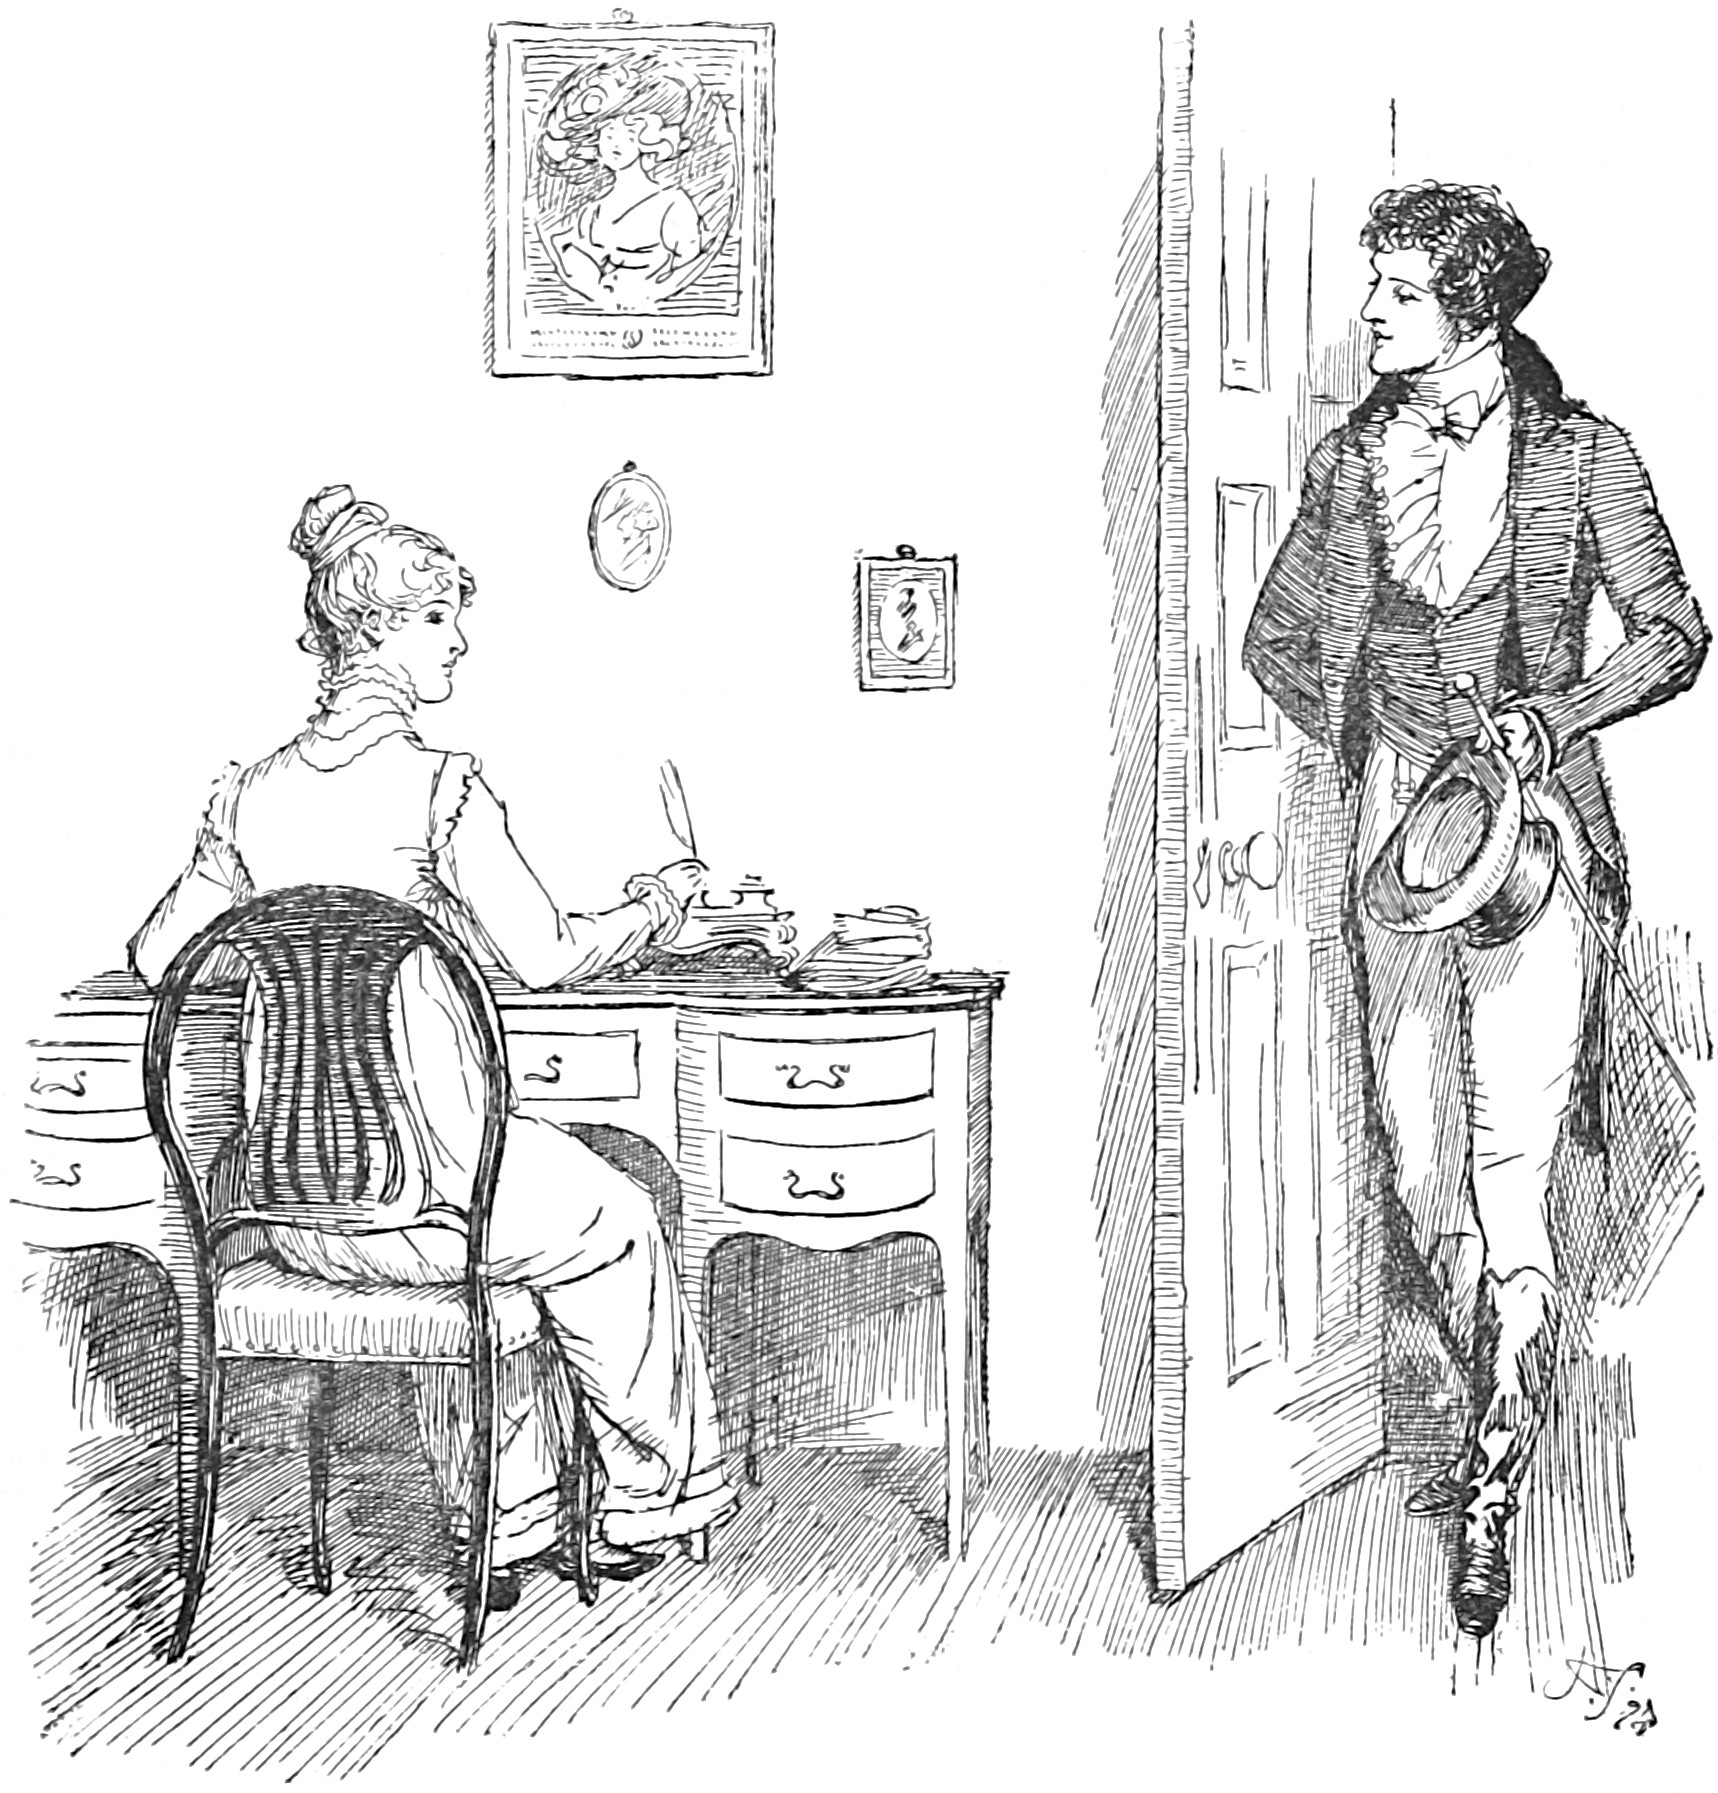
\includegraphics[width=\linewidth]{32top}
\captionlistentry{Headpiece to Chapter \thechapter}
\end{figure}


\lettrine[lines=6,image=true]{initials/chap34w}{hen}  they were gone, Elizabeth, as if intending to exasperate herself as much as possible against Mr Darcy, chose for her employment the examination of all the letters which Jane had written to her since her being in Kent. They contained no actual complaint, nor was there any revival of past occurrences, or any communication of present suffering. But in all, and in almost every line of each, there was a want of that cheerfulness which had been used to characterize her style, and which, proceeding from the serenity of a mind at ease with itself, and kindly disposed towards everyone, had been scarcely ever clouded. Elizabeth noticed every sentence conveying the idea of uneasiness, with an attention which it had hardly received on the first perusal. Mr Darcy's shameful boast of what misery he had been able to inflict gave her a keener sense of her sister's sufferings. It was some consolation to think that his visit to Rosings was to end on the day after the next, and a still greater that in less than a fortnight she should herself be with Jane again, and enabled to contribute to the recovery of her spirits, by all that affection could do.

She could not think of Darcy's leaving Kent without remembering that his cousin was to go with him; but Colonel Fitzwilliam had made it clear that he had no intentions at all, and, agreeable as he was, she did not mean to be unhappy about him.

While settling this point, she was suddenly roused by the sound of the door-bell; and her spirits were a little fluttered by the idea of its being Colonel Fitzwilliam himself, who had once before called late in the evening, and might now come to inquire particularly after her. But this idea was soon banished, and her spirits were very differently affected, when, to her utter amazement, she saw Mr Darcy walk into the room. In a hurried manner he immediately began an inquiry after her health, imputing his visit to a wish of hearing that she were better. She answered him with cold civility. He sat down for a few moments, and then getting up walked about the room. Elizabeth was surprised, but said not a word. After a silence of several minutes, he came towards her in an agitated manner, and thus began:—

»In vain have I struggled. It will not do. My feelings will not be repressed. You must allow me to tell you how ardently I admire and love you.«

Elizabeth's astonishment was beyond expression. She stared, coloured, doubted, and was silent. This he considered sufficient encouragement, and the avowal of all that he felt and had long felt for her immediately followed. He spoke well; but there were feelings besides those of the heart to be detailed, and he was not more eloquent on the subject of tenderness than of pride. His sense of her inferiority, of its being a degradation, of the family obstacles which judgment had always opposed to inclination, were dwelt on with a warmth which seemed due to the consequence he was wounding, but was very unlikely to recommend his suit.

In spite of her deeply-rooted dislike, she could not be insensible to the compliment of such a man's affection, and though her intentions did not vary for an instant, she was at first sorry for the pain he was to receive; till roused to resentment by his subsequent language, she lost all compassion in anger. She tried, however, to compose herself to answer him with patience, when he should have done. He concluded with representing to her the strength of that attachment which in spite of all his endeavours he had found impossible to conquer; and with expressing his hope that it would now be rewarded by her acceptance of his hand. As he said this she could easily see that he had no doubt of a favourable answer. He \textit{spoke} of apprehension and anxiety, but his countenance expressed real security. Such a circumstance could only exasperate farther; and when he ceased the colour rose into her cheeks and she said,—

»In such cases as this, it is, I believe, the established mode to express a sense of obligation for the sentiments avowed, however unequally they may be returned. It is natural that obligation should be felt, and if I could \textit{feel} gratitude, I would now thank you. But I cannot—I have never desired your good opinion, and you have certainly bestowed it most unwillingly. I am sorry to have occasioned pain to anyone. It has been most unconsciously done, however, and I hope will be of short duration. The feelings which you tell me have long prevented the acknowledgment of your regard can have little difficulty in overcoming it after this explanation.«

Mr Darcy, who was leaning against the mantel-piece with his eyes fixed on her face, seemed to catch her words with no less resentment than surprise. His complexion became pale with anger, and the disturbance of his mind was visible in every feature. He was struggling for the appearance of composure, and would not open his lips till he believed himself to have attained it. The pause was to Elizabeth's feelings dreadful. At length, in a voice of forced calmness, he said,—

»And this is all the reply which I am to have the honour of expecting! I might, perhaps, wish to be informed why, with so little \textit{endeavour} at civility, I am thus rejected. But it is of small importance.«

»I might as well inquire,« replied she, »why, with so evident a design of offending and insulting me, you chose to tell me that you liked me against your will, against your reason, and even against your character? Was not this some excuse for incivility, if I \textit{was} uncivil? But I have other provocations. You know I have. Had not my own feelings decided against you, had they been indifferent, or had they even been favourable, do you think that any consideration would tempt me to accept the man who has been the means of ruining, perhaps for ever, the happiness of a most beloved sister?«

As she pronounced these words, Mr Darcy changed colour; but the emotion was short, and he listened without attempting to interrupt her while she continued,—

»I have every reason in the world to think ill of you. No motive can excuse the unjust and ungenerous part you acted \textit{there}. You dare not, you cannot deny that you have been the principal, if not the only means of dividing them from each other, of exposing one to the censure of the world for caprice and instability, the other to its derision for disappointed hopes, and involving them both in misery of the acutest kind.«

She paused, and saw with no slight indignation that he was listening with an air which proved him wholly unmoved by any feeling of remorse. He even looked at her with a smile of affected incredulity.

»Can you deny that you have done it?« she repeated.

With assumed tranquillity he then replied, »I have no wish of denying that I did everything in my power to separate my friend from your sister, or that I rejoice in my success. Towards \textit{him} I have been kinder than towards myself.«

Elizabeth disdained the appearance of noticing this civil reflection, but its meaning did not escape, nor was it likely to conciliate her.

»But it is not merely this affair,« she continued, »on which my dislike is founded. Long before it had taken place, my opinion of you was decided. Your character was unfolded in the recital which I received many months ago from Mr Wickham. On this subject, what can you have to say? In what imaginary act of friendship can you here defend yourself? or under what misrepresentation can you here impose upon others?«

»You take an eager interest in that gentleman's concerns,« said Darcy, in a less tranquil tone, and with a heightened colour.

»Who that knows what his misfortunes have been can help feeling an interest in him?«

»His misfortunes!« repeated Darcy, contemptuously,—»yes, his misfortunes have been great indeed.«

»And of your infliction,« cried Elizabeth, with energy; »You have reduced him to his present state of poverty—comparative poverty. You have withheld the advantages which you must know to have been designed for him. You have deprived the best years of his life of that independence which was no less his due than his desert. You have done all this! and yet you can treat the mention of his misfortunes with contempt and ridicule.«

»And this,« cried Darcy, as he walked with quick steps across the room, »is your opinion of me! This is the estimation in which you hold me! I thank you for explaining it so fully. My faults, according to this calculation, are heavy indeed! But, perhaps,« added he, stopping in his walk, and turning towards her, »these offences might have been overlooked, had not your pride been hurt by my honest confession of the scruples that had long prevented my forming any serious design. These bitter accusations might have been suppressed, had I, with greater policy, concealed my struggles, and flattered you into the belief of my being impelled by unqualified, unalloyed inclination; by reason, by reflection, by everything. But disguise of every sort is my abhorrence. Nor am I ashamed of the feelings I related. They were natural and just. Could you expect me to rejoice in the inferiority of your connections?—to congratulate myself on the hope of relations whose condition in life is so decidedly beneath my own?«

Elizabeth felt herself growing more angry every moment; yet she tried to the utmost to speak with composure when she said,—

»You are mistaken, Mr Darcy, if you suppose that the mode of your declaration affected me in any other way than as it spared me the concern which I might have felt in refusing you, had you behaved in a more gentlemanlike manner.«

She saw him start at this; but he said nothing, and she continued,—

»You could not have made me the offer of your hand in any possible way that would have tempted me to accept it.«

Again his astonishment was obvious; and he looked at her with an expression of mingled incredulity and mortification. She went on,—

»From the very beginning, from the first moment, I may almost say, of my acquaintance with you, your manners impressing me with the fullest belief of your arrogance, your conceit, and your selfish disdain of the feelings of others, were such as to form that groundwork of disapprobation, on which succeeding events have built so immovable a dislike; and I had not known you a month before I felt that you were the last man in the world whom I could ever be prevailed on to marry.«

»You have said quite enough, madam. I perfectly comprehend your feelings, and have now only to be ashamed of what my own have been. Forgive me for having taken up so much of your time, and accept my best wishes for your health and happiness.«

And with these words he hastily left the room, and Elizabeth heard him the next moment open the front door and quit the house. The tumult of her mind was now painfully great. She knew not how to support herself, and, from actual weakness, sat down and cried for half an hour. Her astonishment, as she reflected on what had passed, was increased by every review of it. That she should receive an offer of marriage from Mr Darcy! that he should have been in love with her for so many months! so much in love as to wish to marry her in spite of all the objections which had made him prevent his friend's marrying her sister, and which must appear at least with equal force in his own case, was almost incredible! it was gratifying to have inspired unconsciously so strong an affection. But his pride, his abominable pride, his shameless avowal of what he had done with respect to Jane, his unpardonable assurance in acknowledging, though he could not justify it, and the unfeeling manner which he had mentioned Mr Wickham, his cruelty towards whom he had not attempted to deny, soon overcame the pity which the consideration of his attachment had for a moment excited.

She continued in very agitating reflections till the sound of Lady Catherine's carriage made her feel how unequal she was to encounter Charlotte's observation, and hurried her away to her room.